\chapter{Introducción específica} % Main chapter title

\label{Chapter2}

%----------------------------------------------------------------------------------------
%	SECTION 1
%----------------------------------------------------------------------------------------
En el presente capítulo se introducen las tecnologías más importantes involucradas en el desarrollo del emulador on-line y las características de funcionamiento y de diseño.

\section{Plataforma web}
\label{sec:Plataforma web}

Las aplicaciones web son provistas por un servidor web y pueden ser accedidas por los usuarios que se conecten a través de internet desde cualquier lugar mediante un navegador web \citep{NavegadorWeb}. Además, presentan la arquitectura cliente/servidor en donde un cliente o navegador web realiza peticiones al servidor y en consecuencia el servidor envía la respuesta de regreso. 
En la figura \ref{fig:ClienteServidor} se muestra el esquema del modelo cliente/servidor.

\begin{figure}[ht]
	\centering
	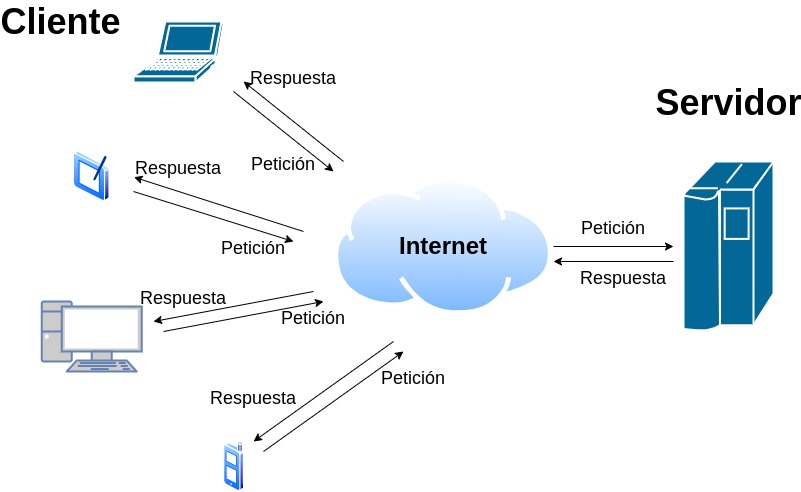
\includegraphics[scale=.45]{./Figures/EsquemaCliente_Servidor.jpg}
	\caption{Esquema modelo cliente/servidor.}
	\label{fig:ClienteServidor}
\end{figure}

Las razones por las que se optó por la tecnologia web se debe a las potenciales ventajas que presentan, de las cuales las más importantes son:

\begin{itemize}
	\item No es necesario instalar nada en la computadora del usuario.
	\item No consumen los recursos del ordenador.
	\item No se encuentra limitado a un lugar físico específico para acceder y utilizar las capacidades de emulación.
	\item No obliga al usuario a usar un determinado sistema operativo, ya que se puede ejecutar en todos los dispositivos con acceso a un navegador web y una conexión a internet.
\end{itemize}

En el desarrollo web, el \textit{frontend} es la parte del software que interactúa con el usuario y el \textit{backend} es la parte lógica que se encarga de tomar los datos, procesarlos y devolverlos al \textit{front end}.

En la figura \ref{fig:frontBack} se muestra un esquema con las tecnologías
web usadas en el presente trabajo.

\begin{figure}[ht]
	\centering
	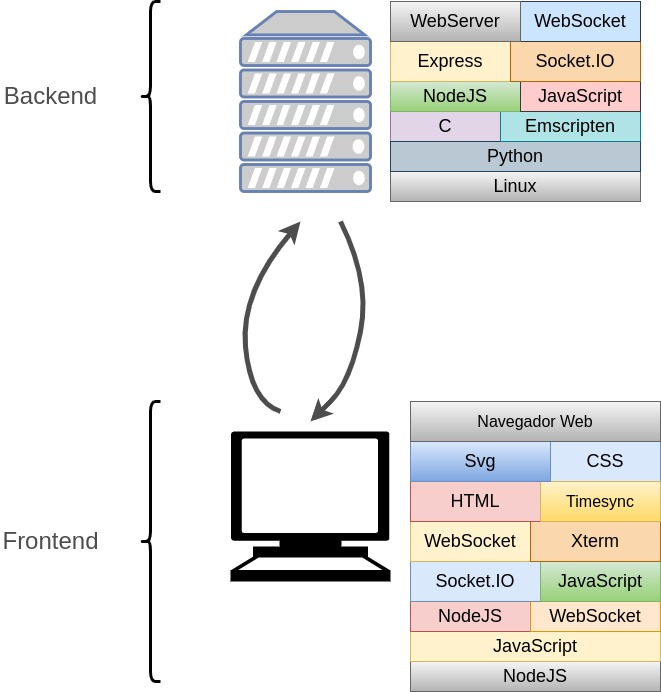
\includegraphics[scale=.57]{./Figures/FrontendBackend.jpg}
	\caption{Esquema de las tecnologías que se usaron en el trabajo.}
	\label{fig:frontBack}
\end{figure}

\hfill \break
\hfill \break
\hfill \break
\hfill \break

\subsection{Frontend}
\label{subsec:Frontend}

Se describen brevemente las principales tecnologías que se usaron en esta parte del diseño de software.

\begin{itemize}
	\item JavaScript \citep{JavaScript}: es un lenguaje de programación que se ejecuta del lado del cliente en el navegador, o bien del lado del servidor mediante motores como NodeJS \citep{NodeJS}. En el caso del lado del cliente, permite crear páginas web dinámicas y también responder a eventos causados por el propio usuario tales como modificaciones del DOM, de la sigla en inglés  \textit{Document Object Model} \citep{DOM}. Por consiguiente, el desarrollo con JavaScript en el frontend permitió cargar y ejecutar los archivos resultantes generados por el compilador en el navegador. Asimismo, es el responsable de configurar el entorno necesario para ejecutar el emulador web y proporcionar la interfaz de usuario para la interacción. Además, en el backend fue útil para gestionar la comunicación y la interacción entre los diferentes componentes, permitiendo la transferencia de datos y el flujo de información dentro de la plataforma web.

	\item NodeJS \citep{NodeJS}: 
es un entorno de ejecución de JavaScript cuyo propósito es el desarrollo de aplicaciones web y servicios del lado del servidor. También, proporciona una arquitectura orientada a eventos y no bloqueante. 
De manera que, en el contexto del frontend, se utilizó como parte del flujo de trabajo de desarrollo, incluyendo la gestión de dependencias, automatización de tareas de compilación, pruebas y despliegue. Mientras tanto, en el backend, fue aprovechado para desarrollar las rutas, controladores y manejar la lógica de la aplicación en respuesta a las solicitudes entrantes y el envío de respuestas.

	\item HTML \citep{HTML}: de la sigla en inglés \textit{Lenguaje de Marcas de Hipertexto, del inglés HyperText Markup Language}, es el lenguaje de marcas que sirve para etiquetar contenido y visualizarlos en el navegador web.
	Este lenguaje es sencillo de aprender y es fácil de interpre­tar tanto por humanos como por máquinas.  En el desarrollo, se utilizó para crear los elementos visuales de la interfaz de usuario, como los botones, lista desplegable, pantallas de visualización, y otros componentes necesarios para interactuar con el emulador web.

	\item CSS \citep{CSS}: de la sigla en inglés \textit{Cascading Style Sheets},
	es un lenguaje de diseño gráfico que permite definir estilos, colores, formato, tamaño, tipo de letra del texto, posición de cada elemento dentro de la página, etc. Es la mejor forma de separar los contenidos y es necesario para crear páginas web complejas. El desarrollo con CSS ayudó a controlar la presentación visual y el estilo de la plataforma.

    \item SVG \citep{SVG}: de la sigla en inglés \textit{Scalable Vector Graphics}, es un formato de gráficos vectoriales bidimensionales con una base matemática que pueden modificarse según se necesite. Las imágenes creadas con este formato se pueden escalar y hacer zoom de forma arbitraria sin pérdida de resolución debido a que no están formadas por píxeles. Además, esta basado en el lenguaje de marcado extensible XML \citep{XML} y es un formato muy útil para ser utilizado en entornos web. 
Para el desarrollo del diseño de la interfaz fue ideal el uso de este tipo de formato para evitar que las imagenes se deformen y también, ofrecer una experiencia visual interactiva.

    \item Xterm \citep{Xterm}: es un componente escrito en TypeScript \citep{TypeScript} que permite que una aplicación pueda usar terminales emuladas con todas sus funciones en el navegador web. 
En el desarrollo del emulador web, se utilizó esta tecnología en la interfaz de usuario para visualizar la salida de la terminal.

    \item WebSocket \citep{WebSocket}: esta tecnología permite la comunicación bidireccional entre el cliente y el servidor, trabaja sobre el protocolo TCP/IP y también, es una especificación de protocolo de HTML5, de la sigla en inglés \textit{HyperText Markup Language, versión 5} \citep{HTML5}. 
Se utilizó WebSocket para establecer una conexión entre el frontend y el backend, y de esta manera, enviar los datos desde el backend al frontend para mostrarlos en la terminal serial. Es decir, permite que los datos de la terminal serial se reflejen de manera dinámica en la interfaz de usuario del frontend.
       
    \item Socket.IO \citep{Socket}: es una biblioteca de Javascript que usa websocket para la comunicación bidireccional y para la baja latencia. También, está basada en el manejo de eventos entre un cliente y un servidor. El desarrollo con esta tecnología permitió facilitar la comunicación en tiempo real entre el cliente y el servidor para la la terminal serial.
    
    \item Timesync \citep{Timesync}: es una biblioteca de JavaScript que se usa para sincronizar temporizadores en una aplicación y, además, las aplicaciones cliente sincronizan el tiempo con el servidor, ya sea a través de peticiones HTTP o WebSockets. El desarrollo de la plataforma web con esta tecnología aseguró que los eventos y acciones ocurran en el momento exacto tanto en el cliente como en el servidor.
    
     \item Mocha \citep{Mocha}: es un marco de trabajo para pruebas de JavaScript que tiene funciones que se ejecutan en NodeJS y en el navegador web. En consecuencia, hace que las pruebas asincrónicas sean simples. Asimismo, Las pruebas se ejecutan en serie y se realiza el envío de excepciones aún no detectadas a los casos de prueba correctos.
El uso de este marco de trabajo permitió hacer pruebas sobre la interfaz de usuario de la plataforma.
     
     \item Chai \citep{Chai}: es una biblioteca de aserciones que puede usarse con cualquier marco de pruebas de Javascript. Asimismo, tiene varias interfaces: \textit{assert}, \textit{expect} y \textit{should}, que permiten al desarrollador elegir cuál usar. Chai se utiliza en las pruebas del emulador web para  verificar el comportamiento esperado de las funciones, componentes y datos generados por el emulador. 
   
\end{itemize}


\subsection{Backend}

Se describen brevemente las principales tecnologías que se usaron en el backend.

\begin{itemize}
	\item Emscripten \citep{Emscripten}: es un compilador que traduce la mayor parte del lenguaje LLVM, de la sigla en inglés \textit{Low Level Virtual Machine} \citep{LLVM}, a JavaScript. De esta forma, permite ejecutar el código de varios lenguajes de programación en los navegadores actuales.
Emscripten compila C y C++ en WebAssembly \citep{WebAssembly} mediante LLVM y Binaryen \citep{Binaryen}. La salida de Emscripten puede ejecutarse en la web y en NodeJS.
El uso de esta herramienta tuvo por objetivo el compilar el código escrito en C, a WebAssembly (Wasm) y JavaScript.	Esto permitió ejecutar aplicaciones nativas en la web sin necesidad de plugins o complementos adicionales.

	\item Python \citep{Python}:  es un poderoso y popular lenguaje de programación multiplataforma de código abierto. Se caracteriza por su sencillez y su gran potencia para el tratamiento de datos en el lado del servidor. En el emulador web, Python se utilizó para escribir scripts que realicen tareas específicas, como la configuración, inicialización y depuración. De esta manera, facilitó el desarrollo.
    
    \item Express \citep{Express}: es un marco de aplicaciones web en el backend para NodeJS. También, está diseñado para crear aplicaciones web y APIs, de la sigla en inglés \textit{application programming interface} \citep{API}. El uso de este framework simplifico el manejo de solicitudes HTTP, la definición de rutas para interactuar con la plataforma web. De manera que, facilitó que el desarrollo del emulador web sea más simple y estructurado.
    
    \item Lenguaje C \citep{LenguajeC}: es de propósito general y es muy popular debido al eficiente código que produce al crear software de sistemas y de aplicaciones. 
    Asimismo, es un lenguaje de tipos de datos estáticos, fuertemente tipado y tiene estructuras típicas de los lenguajes de alto nivel pero, a su vez, tiene construcciones que permiten un control de los lenguajes de bajo nivel. El desarrollo con C fue fundamental, ya que permitió la integración de las sAPI de la CIAA en el desarrollo del emulador web.

    
    \item Check \citep{Check}: es una biblioteca de pruebas unitarias para el lenguaje de programación C que proporciona un conjunto de macros y funciones que facilitan la escritura y la ejecución de las pruebas unitarias. Además, provee mecanismos que aislan y ejecutan las pruebas en un entorno controlado y separado, usando suites de pruebas, funciones de inicialización y limpieza. Se utilizó en el emulador web para verificar el correcto funcionamiento de las funciones y componentes implementados en el backend del emulador escritos en lenguaje C.
    
    \item CMocka \citep{CMocka}: es una biblioteca de pruebas unitarias especialmente diseñada para C, destacandose por su capacidad de crear mocks (falsos) y stubs (simulaciones) de funciones. De esta manera se logra probar componentes de código que dependen de funciones externas. Y, además, facilita el aislamiento de las unidades de código y la creación de escenarios de prueba que pueden ser controlados. El uso de esta tecnología permitió simular funciones mediante mocks para controlar el comportamiento de las funciones dependientes y facilitar las pruebas de código que interactúa con dichas funciones.
    
	    \item sAPI CIAA \citep{sAPICIAA}: esta biblioteca escrita en lenguaje C y compatible con C++ implementa una API simple que funciona como una capa de abstracción de hardware para microcontroladores. Es la principal biblioteca del Proyecto CIAA para el desarrollo de aplicaciones en C/C++ en los frameworks Firmware v2\citep{firmwareV2} y Firmware v3\citep{firmwareV3}. 
Para la emulación a nivel de API, se utilizó como base la API de la sAPI v0.6.2 disponible en firmware v3 del Proyecto CIAA \citep{sAPIv0.6.2} y se realizarón las implementaciones necesarias para que funcione en la web, en lugar de funcionar en el hardware de un microcontrolador real.
De esta manera, se proporcionó una interfaz idéntica, permitiendo a los usuarios del emulador programar en la plataforma web de la misma manera que lo harían con la placa EDU-CIAA real, logrando que cualquier programa escrito utilizando la sAPI pueda correr en el emulador.
Cabe destacar que al emular a nivel de sAPI, el usuario no podrá utilizar funciones de bajo nivel de la EDU-CIAA, como ser la biblioteca del fabricante del microcontrolador (LPCopen\citep{lpcopen}), o el acceso directo a registros físicos del microcontrolador.
    
    \item Mbed CLI \citep{MbedCLI}: es una herramienta de línea de comandos que facilita el desarrollo y la gestión de proyectos basados en la plataforma Mbed \citep{ArmMbed}. Incluso, permite realizar tareas como la configuración del entorno de desarrollo, compilación de código, gestión de dependencias y la depuración, permitiendo identificar y resolver problemas en el código. Se reutilizó esta herramienta, ya incluída en el emulador sobre el cual se basó este trabajo, para proporcionar una interfaz de línea de comandos que simplificó las tareas de configuración y construcción del emulador web.
 
    \item SVG EDU-CIAA-NXP \citep{SVGFirmwareV3}: se reutilizaron para el presente trabajo los dibujos de la placa EDU-CIAA-NXP. La reutilización de estos dibujos fueron necesarios para proporcionar al usuario una experiencia visual interactiva.
    
     \item Mbed events \citep{ArmMbed}: es una biblioteca de código que se utiliza en el desarrollo de software embebido para facilitar la gestión de eventos y temporizadores. Para el desarrollo de la plataforma del emulador web se reutilizó esta biblioteca para la creación y gestión de tareas en freeRTOS.
     
\end{itemize}


\section{Herramientas de trabajo}
\label{sec:Herramientas de trabajo}

Se exponen las principales plataformas que se usaron para el desarrollo de este trabajo.

\begin{itemize}
	\item EDU-CIAA-NXP: esta es la plataforma de hardware objetivo a emular del presente trabajo. Es uno de los diseños de hardware del Proyecto CIAA. En particular, el enfoque es ayudar a las Universidades Argentinas a migrar de microcontroladores de 8 bits a modernos microcontroladores de 32 bits al usar una placa diseñada en Argentina con hardware y software abiertos. Estas placas se difundieron en todas las universidades Argentinas con carreras de electrónica y afines, y también, en algunos países limítrofes. 
Se utilizó la placa física para ensayos de comparación entre lo real y el emulador web desarrollado.

	\item Visual Studio Code \citep{VisualStudioCode}: es un editor de código fuente gratuito y de código abierto desarrollado por Microsoft. Incluye soporte para la depuración, control integrado de Git, resaltado de sintaxis, finalización inteligente de código, fragmentos, refactorización de código y muchas otras herramientas más. Se eligio este IDE, de la sigla en inglés Integrated Development Environment \citep{IDE}, por la capacidad de sus herramientas y la simpleza de su editor de código. El uso de este editor facilitó la escritura y el mantenimiento del código del emulador, mejorando la productividad y la calidad del desarrollo.
	
	\item Inkscape \citep{inkscape}: es un editor de gráficos vectoriales que permite crear, editar y modificar gráficos. En el proceso de desarrollo de la interfaz del emulador web se utilizó para diseñar algunos elementos gráficos dentro del dibujo de la placa EDU-CIAA-NXP.

	\item GitHub \citep{GitHub}: es una plataforma de desarrollo colaborativo que permite alojar proyectos utilizando el sistema de control de versiones Git. Se utilizó los servicios de esta plataforma para almacenar y
compartir el código fuente, de manera que se pueda hacer un seguimiento
de las últimas modificaciones realizadas.
	
	\item Travis CI \citep{TravisCI}: es un servicio de integración continua en la nube y es utilizado mayormente para configurar y ejecutar pruebas automatizadas en un entorno controlado y reproducible. Además, se integra con sistemas de control de versiones como GitHub y permite que con cada cambio realizado en el repositorio se ejecuten las pruebas definidas en el script de construcción.
De esta manera, se asegura la calidad del software. Incluso, proporciona informes detallados de las pruebas realizadas y servicio de notificaciones por correo electrónico.

	\item GitLab \citep{GitLab}: es una plataforma web de gestión de repositorios y permite la colaboración en el desarrollo de software. Proporciona un conjunto completo de herramientas para el ciclo de vida del desarrollo de software, por lo tanto, permite configurar pipelines de integración y entrega continua, en consecuencia, automatiza la compilación, las pruebas y el despliegue de software de manera eficiente. Es una alternativa a otras plataformas como GitHub con Travis CI.
	
	\item DigitalOcean \citep{DigitalOcean}: ofrece servicios de infraestructura de computación en la nube, tales como permitir a los usuarios crear y administrar servidores virtuales, conocidos como Droplets. Incluso, ofrece opciones de almacenamiento, configuración de redes privadas virtuales, servicios de bases de datos, entre otros. DigitalOcean se destaca por su enfoque en la simplicidad y la facilidad de uso de su plataforma. El emulador desarrollado en el presente trabajo se encuentra desplegado en el servidor de DigitalOcean.

	
\end{itemize}
